\documentclass[tikz,border=3pt]{standalone}
% common black-and-white style of the diagrams
\usepackage[T1]{fontenc}
\usepackage{mathptmx}
\usepackage{amsmath,amssymb,bm}
\usetikzlibrary{arrows.meta,positioning,fit,calc,backgrounds,shapes.geometric,shapes.misc,patterns}
\tikzset{
  every picture/.style={font=\small, line width=0.5pt},
  >={Latex[length=2.2mm,width=1.5mm]},
  blk/.style={draw, rectangle, fill=white, align=center, inner sep=3pt, minimum height=9mm},
  grp/.style={draw, rectangle, dashed, inner sep=4pt},
  arr/.style={->, line width=0.6pt},
  darr/.style={->, line width=0.6pt, dash pattern=on 3pt off 2pt},
  lbl/.style={font=\footnotesize, align=center},
  ttl/.style={font=\small\bfseries},
}

\AtBeginDocument{\hyphenpenalty=10000 \exhyphenpenalty=10000 \relax}

\begin{document}
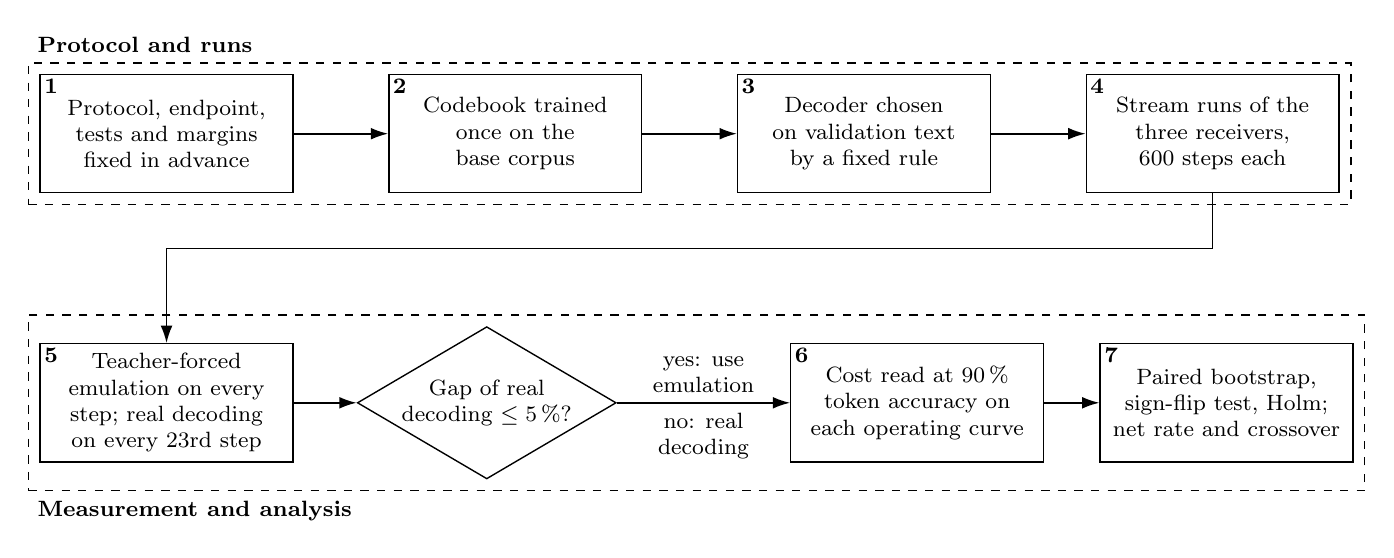
\begin{tikzpicture}[
  font=\footnotesize,
  box/.style={blk, text width=30mm, minimum height=15mm},
  dec/.style={draw, diamond, aspect=1.7, fill=white, align=center, inner sep=0.5pt, text width=22mm},
  num/.style={font=\footnotesize\bfseries, anchor=north west, inner sep=1.5pt},
  node distance=7mm
]
% row 1: fixed before the confirmatory runs
\node[box] (p1) {Protocol, endpoint, tests and margins fixed in advance};
\node[box, right=12mm of p1] (p2) {Codebook trained once on the base corpus};
\node[box, right=12mm of p2] (p3) {Decoder chosen on validation text by a fixed rule};
\node[box, right=12mm of p3] (p4) {Stream runs of the three receivers, 600 steps each};
% row 2: measurement and analysis
\node[box, below=19mm of p1] (m1) {Teacher-forced emulation on every step; real decoding on every 23rd step};
\node[dec, right=8mm of m1] (d) {Gap of real decoding $\le 5$\,\%?};
\node[box, right=22mm of d] (m2) {Cost read at 90\,\% token accuracy on each operating curve};
\node[box, right=of m2] (m3) {Paired bootstrap, sign-flip test, Holm; net rate and crossover};
\foreach \n/\k in {p1/1,p2/2,p3/3,p4/4,m1/5,m2/6,m3/7} { \node[num] at (\n.north west) {\k}; }
\draw[arr] (p1) -- (p2);
\draw[arr] (p2) -- (p3);
\draw[arr] (p3) -- (p4);
\draw[arr] (p4.south) -- ++(0,-7mm) -| (m1.north);
\draw[arr] (m1) -- (d);
\draw[arr] (d) -- node[lbl, above]{yes: use\\ emulation} node[lbl, below]{no: real\\ decoding} (m2);
\draw[arr] (m2) -- (m3);
\node[grp, fit=(p1)(p4)] (g1) {};
\node[grp, fit=(m1)(m3)(d)] (g2) {};
\node[ttl, anchor=south west, font=\footnotesize\bfseries] at (g1.north west) {Protocol and runs};
\node[ttl, anchor=north west, font=\footnotesize\bfseries] at (g2.south west) {Measurement and analysis};
\end{tikzpicture}
\end{document}
